\section{Аналитический раздел}

\subsection{Постановка задачи}

Необходимо разработать систему, которая будет автоматически управлять распределением поездов по платформам на железнодорожной станции, избегая задержек и перегрузок.
Система должна оптимизировать движение поездов с учетом направления и доступных ресурсов станции.

На рисунке \ref{img:A0} приведены IDEF0-схемы для поставленной задачи.
\begin{figure}[h]
	\centering
	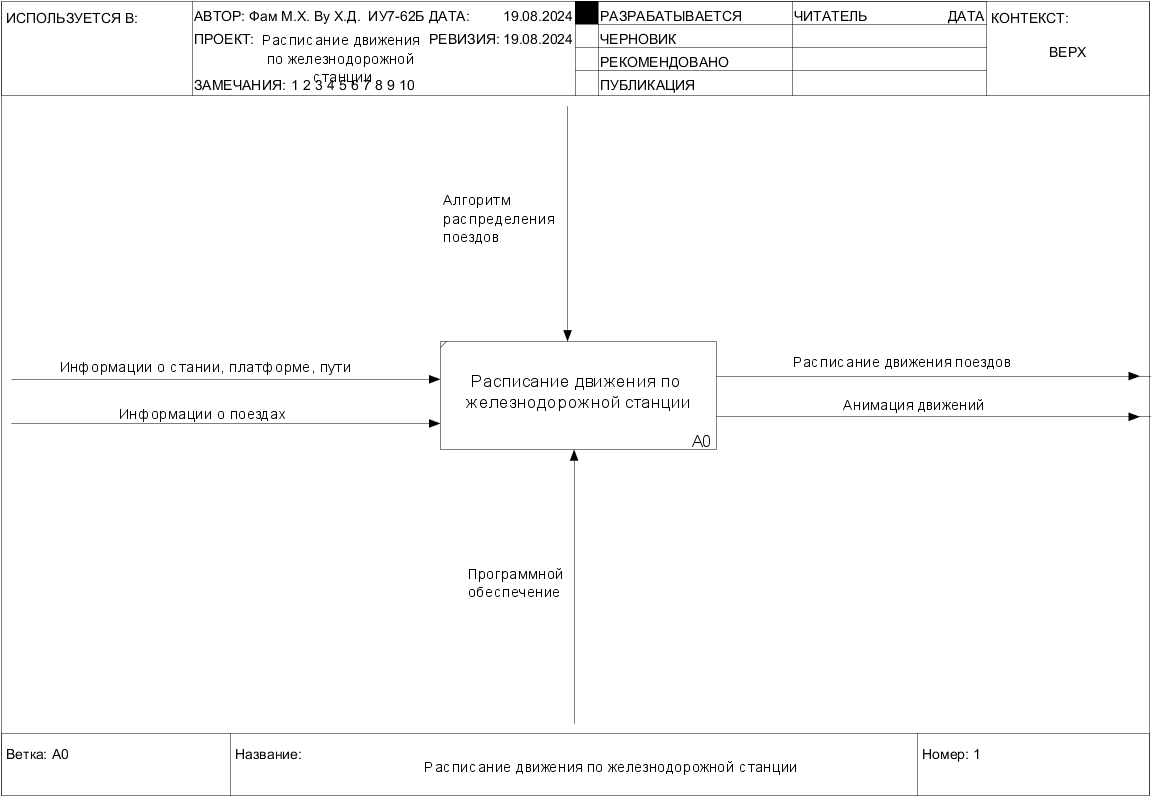
\includegraphics[height=0.45\textheight]{img/idef0/01_A0.png}
	\caption{Контекстная диаграмма (A-0)}
	\label{img:A0}
\end{figure}

\subsection{Формализация данных}

Выделяются следующие сущности, связанные с данной задачей:
\begin{itemize}
	\item станция;
	\item платформа;
	\item путь;
	\item поезд;
\end{itemize}

Информация о каждой сущности проводится в таблице~\ref{tb:data}.

\begin{table}[ht]
	\begin{center}
		\begin{threeparttable}
			\caption{\label{tb:data} Сущности и их описания}
			\begin{tabular}{|c|p{10cm}|}
				\hline
				\textbf{Сущность} & \textbf{Описание} \\ \hline
				Станция & Название, список платформ, расписание \\ \hline
				Платформа & ID, список путей \\ \hline
				Путь & ID, направление, список текущих поездов \\ \hline
				Поезд & ID, рисунок, время отправления, время прибытия, тип, ID платформы, ID пути \\ \hline
			\end{tabular}
		\end{threeparttable}
	\end{center}
\end{table}

\subsection*{Вывод}
В данном разделе была проанализирована предметная область.
Была преведена постановка задачи, формализация данных и построена соотвествующая ER-диаграмма. 
Также описаны системные пользователи.
Проведен анализ баз данных по модели данных и на основе этого анализа была выбрана подходящая модель для решения поставленной задачи.